% Chapter 2
\chapter{理论基础}
\section{音频特征建模基础}
在深度学习领域,音频特征建模常用于语音识别等领域。目前市面常见的虚拟助手:Siri、小爱同学和图灵机器人等,都是构建于音频特征建模的基础上。在音频分类、语言合成和语言认识方面,音频特征建模已经很成熟了。
在深度学习领域,音频特征建模常用于语音识别等领域。目前市面常见的虚拟助手:Siri、小爱同学和图灵机器人等,都是构建于音频特征建模的基础上。在音频分类、语言合成和语言认识方面,音频特征建模已经很成熟了。基于音频处理库——Librosa ,本部分主要介绍音频特征建模的理论基础:数字信号处理、滤波器和 Mel 图\cite{mcfee2015librosa}

\begin{figure}[h]
  \centering
  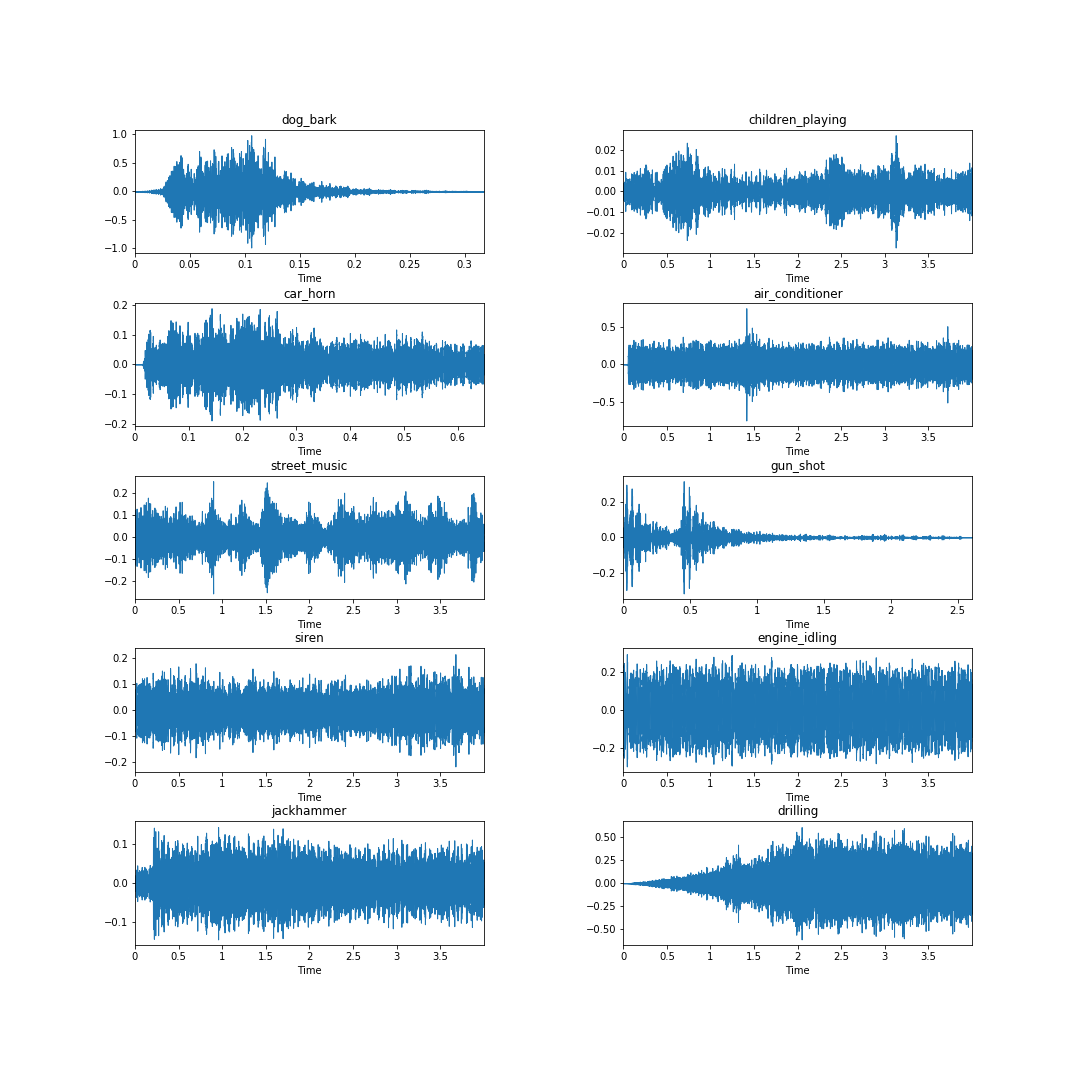
\includegraphics[width=0.7\textwidth]{figures/基础音频.png}
  \caption{常见音频的波形图}
  \label{fig:boxingtu}
\end{figure}

\subsection{从原始音频说起}
常见的音频主要是利用手机麦克风,在40kHz左右的采样频率下进行收集的。因此呈现在 wav 文件中常常是以一维的格式利用扬声器进行输出。从人眼观察的角度来看,音频样本具有着一定的周期性和特征性,但是更精细的信息都是人眼无法去分别出来的,图图\ref{fig:boxingtu}中有个十种音频信号的波形图,通过肉眼观察,引擎声、报警器声和空调声看上去非常的相似。以下音频信号的概念是常见用于描述波形图的特征的术语。
\begin{enumerate}
  \item \textbf{采样和采样频率}:在音频信号处理中,采样是将连续信号按一定规律记录信号使之成为一组离散值而采样频率就是这个采样的规律即一定时间内采样的个数。一般常见手机麦克风的采样频率在40kHz左右。 
  \item \textbf{幅值}: 音频波形的幅度是固定时间内波形变化的量度。幅度的另一个常用定义是变量的极差的大小。一般为了比较相对度的大小,系统会在音频处理种把幅度分量进行归一化处理。
      \begin{figure}[h]
      \centering
      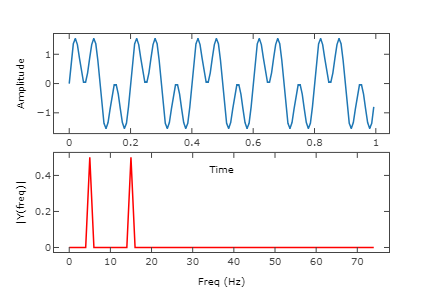
\includegraphics[width=0.7\textwidth]{figures/傅里叶变换图片.png}
      \caption{傅里叶变换示例}
      \label{fig:fuliye}
    \end{figure}
  \item \textbf{傅里叶变换}:原始声音波形往往只能看到其随时间变化规律,而看不出来其频率的变化规律。傅里叶变换就是为了展示其频率变化的一种方法。
        \begin{equation}
         F(w) = \digamma[f(t)] = \int_{-\infty}^{ +\infty} f(t)e^{-iwt} dx
         \label{eq:2.1}
        \end{equation}
        
    傅里叶变换的理论基础是将所有信号看作任意多个三角函数的叠加。因此傅里叶变换是一种将信号投影到三角函数(基)的方法。公式\eqref{eq:2.1}中w表示频率,t表示时间,\eqref{eq:2.1}中将信号表示为三角基函数的叠加。
    对于一个非周期信号,可以将非周期信号看成一个周期信号的一部分。即:傅里叶变换当周期足够大,就会退化为一般情况下的信号函数。因此傅里叶级数退化为:
    \begin{equation}
        f(t) = \sum_{k=-\infty}^{\infty} C_k e^{2\pi(K/T)t}
    \end{equation}
    
    其中\(C_k\)为傅里叶级数,其表示为:
    \begin{equation}
        C_k  = \frac{1}{T}\int_{0}^{T} e^{-2\pi i(\frac{k}{T})t}f(t) d t
        = \frac{1}{T}\int_{-\frac{2}{T}}^{-\frac{2}{T}} e^{-2\pi i(\frac{k}{T})t}f(t) d t
    \end{equation}
    图\ref{fig:fuliye}是利用matlab生成的周期音频信号。上图是一个周期音频信号,下图是该信号的变换结果。

    \item \textbf{周期图}:周期图是基于傅里叶变换的方法。它对音频信号直接做傅里叶变换并且进行平方,如公式\ref{eq:2.4}:
        \begin{equation}
            S_{pre}(w) = \frac{1}{N}|c_k|^2
            \label{eq:2.4}
        \end{equation}
    其中\(C_k\)是傅里叶级数。周期图代表了一个音频在频率方向上密度的估计,即图\ref{fig:zhouqitu}表示的是图\ref{fig:fuliye}中音频信号的周期图。
    \begin{figure}[h]
      \centering
      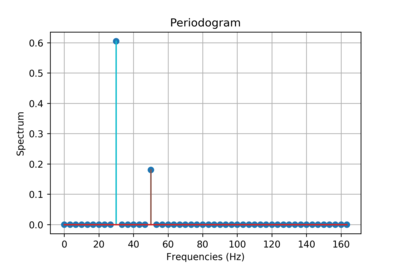
\includegraphics[width=0.7\textwidth]{figures/周期图图片.png}
      \caption{周期图示例}
      \label{fig:zhouqitu}
    \end{figure}
    \item \textbf{梅尔倒频谱系数}:由于人耳对等距离音高感官并不是非线性的。在1980年Davis和Mermelstei\cite{zheng2001comparison}提出一种定义:将1000Hz 且比人类听觉阈值高40分贝高的音频信号定义为1000mels。当频率大于500Hz时,每当人耳感觉到相同的音高变化量时,所需的频率变化就会随着频率的增加而变得越来越大。 
            \begin{equation}
            m = 2595\log_{10}{(1+\frac{f}{700})}
            \label{eq:2.4}
        \end{equation}
    图\ref{fig:mel1}是频率到Mel的映射关系图。从图中可以看到,在频率较低时,Mel随频率变化较快;当频率较高时,斜率变小,变化缓慢\cite{zheng2001comparison}。
     \begin{figure}[h]
      \centering
      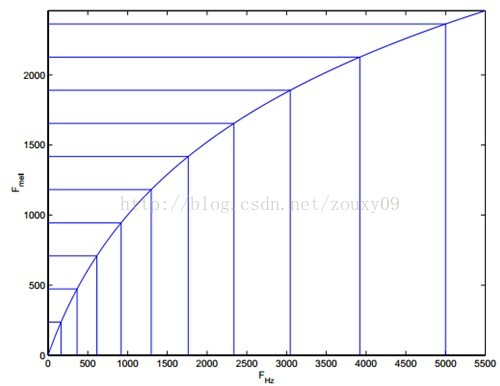
\includegraphics[width=0.7\textwidth]{figures/mel1.jpg}
      \caption{频率:Mel 关系示意图}
      \label{fig:mel1}
    \end{figure}
\end{enumerate}

\subsection{音频特征提取之Mel图}
音频特征提取的一个重要方面就是:梅尔频谱系数(MFCC)的计算,而利用MFCC可以求出Mel图。Mel图与其他一般的音频特征提取方法相比共有以下优势:
\begin{enumerate}
    \item 对于音频的特征进行了去除相关度并进行压缩,更加方便后续的处理。
    \item 适合数据量更小的样本集。
    \item MFCC具有低维度,在频谱上显示的更加平整。
\end{enumerate}
MFCC实现的基本流程图如下图\ref{fig:MFCC},按照预加重、分频加窗、离散傅里叶变换和三角空间滤波、离散余弦变换共五步。
     \begin{figure}[h]
      \centering
      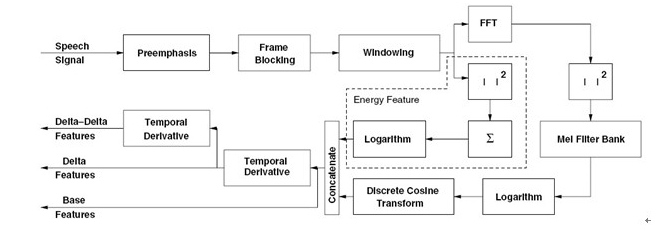
\includegraphics[width=\textwidth]{figures/MFCC.jpg}
      \caption{MFCC实现流程图}
      \label{fig:MFCC}
    \end{figure}
\begin{enumerate}
    \item \textbf{预加重}:由于音频信号在发声过程中会受到嘴唇等身体部位的干扰,需要通过一种高通滤波器来强化高频部分。这样处理后的音频信号会显示的更加平坦,滤波公式为公式\ref{eq:hz}
    \begin{equation}
        H(Z) = 1 - \mu z^{-1}
        \label{eq:hz}
    \end{equation}
    \item \textbf{分帧加窗}:由于手机的采样频率是44.1KHz,即每秒采样44.1K个点,而一般采样的音频频率为22kHz。又因为一个标准帧的长度为25ms。所以每帧有\(22000*0.025 = 550\)个采样点。分帧操作就是对每帧按照10ms的跨度进行拆分。假设声音信号为\(s(n)\),完成分帧操作后为\(s_i(n)\);
    \item \textbf{离散傅里叶变换}:对\(s_i(n)\)做离散傅里叶变换得到\(S_i(k)\),对应的功率密度为\(P_i(k)\);
    \begin{equation}
        S_i(k) = \sum_{n=1}^N s_i(n)h(n)e^{-j2{\pi}kn/N}
    \end{equation}
    \begin{equation}
        P_i(k) = \frac{1}{N}|S_i(k)|^2
    \end{equation}
    对分帧后的数据还需要按帧乘以汉明窗。这种方法可以显著提高帧左右段的连续性,实现公式如下
    \begin{equation}
        S_i(k) = S_i(k)\times W_i(k)
    \end{equation}
    \begin{equation}
        W_i(k,a) = (1-a)-a\times \cos{\frac{2\pi n}{N-1}}
    \end{equation}
    这里的a一般取为0.5
    \begin{figure}[h]
      \centering
      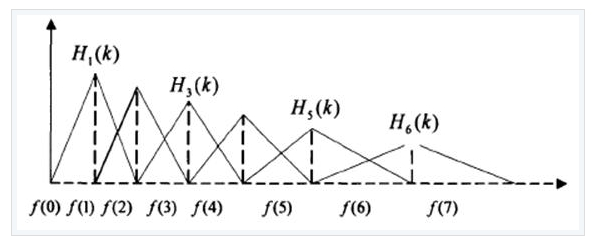
\includegraphics[width=\textwidth]{figures/三角滤波器.jpg}
      \caption{三角滤波器组的设置}
      \label{fig:sanjiao}
    \end{figure}
    \item \textbf{三角空间滤波}:通常使用26个左右的三角滤波器,对\(P_i(k)\)进行滤波,根据公式\ref{eq:2.4},可以求出MEL最大为\(f_{max}[mel] = 2146.1mel\),由于三角空间滤波的设置往往是等间隔的处理,所以其频率的间隔为公式\ref{eq:mel}
    \begin{equation}
        \delta = \frac{f_{max}}{\kappa+1}=93.3 mel
        \label{eq:mel}
    \end{equation}
    同时可对相邻三角空间滤波的上限频率进行设置
    \begin{equation}
        c(l) = h(l-1)=o(l+1)
    \end{equation}
    具体如图\ref{fig:sanjiao}所示

    \item \textbf{离散余弦轩变换}:在求离散余弦变换前需要计算每个滤波器组输出的对数能量
    \begin{equation}
        s(m) = ln(\sum_{k=0}^{N-1}|X_a(k)|^2H_m(k))
    \end{equation}
    其中\(0\le m \le M\),之后利用DCT求得MFCC系数:
    \begin{equation}
        C(k) = \sum_{m=0}^{n-1}s(m)\cos{\frac{\pi k(m-0.5)}{M}}
    \end{equation}
\end{enumerate}
由此对图\ref{fig:fuliye}进行mel图谱的构建,其结果如图\ref{fig:Mel}所示
     \begin{figure}[h]
      \centering
      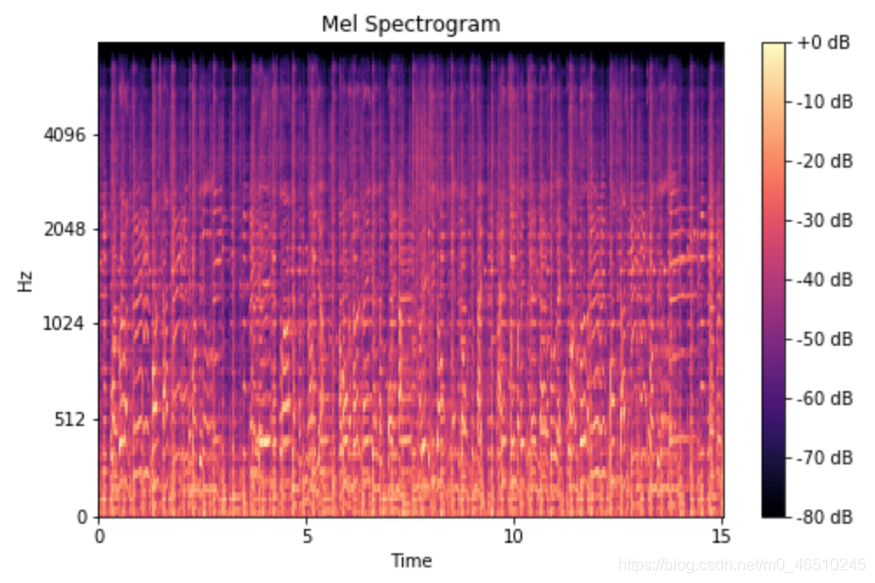
\includegraphics[width=\textwidth]{figures/melPic.png}
      \caption{Mel图}
      \label{fig:Mel}
    \end{figure}
\section{音频数据增强}
\subsection{概述}
音频数据增强最早来自于图像神经网络中的图像增强方法,两者的目的都是为了拓展训练集并鼓励系统对增强过程中的转换保持不变。作为一种补充措施,对系统在转换后的输入上的预测进行学习可以提高针对系统未学习到的样本的鲁棒性。 

在音频数据增强领域,现今的研究成果已经硕果累累了。2013年,Jaitly和Hinton \cite{Jaitly2013VocalTL}率先使用了保留标签的音频转换来进行语音识别。他们发现,在训练和测试时间进行mel滤波之前,频谱图的音调移位会使电话错误率从21.6%降低到20.5%,并报告称按时间或频率维度缩放mel频谱,或者根据扰动的LPC系数构造示例都无济于事。同时,Kanda等人的研究成果\cite{kanda2013elastic}表明,将音调移位与时间拉伸和随机频率失真相结合可将字错误减少10%,而音调移位被证明是最有益的,并且三种失真方法的效果几乎呈线性相加。Xiaodong Cui等人\cite{cui2015data}实现了将音高转换与在特征空间中将语音转换为其他说话者语音的方法结合起来的方法。

在这些研究的基础上,本研究可以确定音频数据增强在提高模型系统性能,避免过度拟合从而提高其通用性。

\subsection{常用的音频数据增强方法介绍及展示}
现今常用的数据增强方法有:加入高斯白噪音、音调转换、时间拉伸、时间平移以及同类音频叠加等。因此本文利用github上的音频数据增强库:audiomentations,展示一些常用的音频数据增强方法,并分析它们的影响。
     \begin{figure}[h]
      \centering
      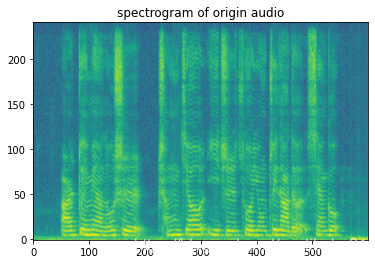
\includegraphics[width=0.5\textwidth]{figures/oasg.png}
      \caption{原始信号的频谱图}
      \label{fig:oasg}
    \end{figure}

按照第一部分介绍的音频特征建模技术,音频数据增强的方法可以用于处理展示频谱图和梅尔频谱图。因为梅尔频谱图需要构建复杂的三角滤波器组,所以本文用频谱图来分析展示数据增强方法,以及这种处理方法的影响。原始信号的频谱图展示如图\ref{fig:oasg}:

分别对原始信号做时间平移、时间拉伸和添加白噪音操作其频谱图变化如图:
    \begin{figure}[h]
      \centering
      \begin{subfigure}{0.3\textwidth}
        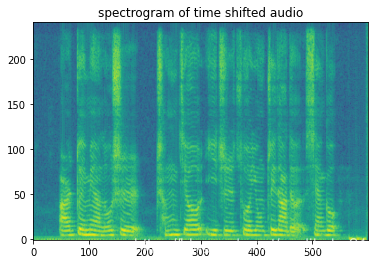
\includegraphics[width=\linewidth]{figures/oats.png}
        \caption{时间平移}
        \label{fig:oats}
      \end{subfigure}
      \begin{subfigure}{0.3\textwidth}
        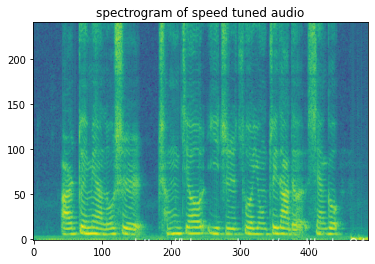
\includegraphics[width=\linewidth]{figures/oast.png}
        \caption{时间拉伸}
        \label{fig:oast}
      \end{subfigure}
        \begin{subfigure}{0.3\textwidth}
        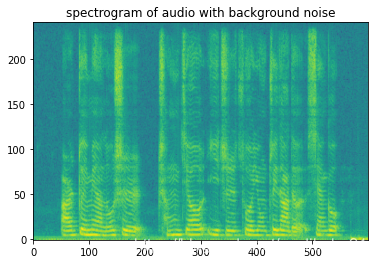
\includegraphics[width=\linewidth]{figures/oabn.png}
        \caption{添加白噪音}
        \label{fig:oabn}
      \end{subfigure}
      \caption{音频数据增强后的频谱图}
      \label{fig:multi-image}
    \end{figure}
    
在audiomentations库中,还有剪切样本、频段屏蔽、质量压缩等音频增强技术的实现。而这些音频增强的方法在最终的模型的影响,将在后面的实验设计过程中进行分析。
\section{迁移学习}
迁移学习是一种微调预训练模型,并快速标记适合的数据的深度学习方法。它与从零开始的深度学习训练相比,微调模型需要更少的标记数据,可以更快的实现训练。
许多迁移学习任务的方法主要有:(i)从一个预先训练的模型开始,(ii)移除特定于任务的顶层,(iii)作为特征提取器对目标任务的底层进行微调。通过这种方法,迁移学习系统可以实现特定任务的特征提取,而本文就采取利用Youtube数据训练的类神经网络VGGish实现基于咳嗽音频的特征提取。
\subsection{研究现状}
Donahue等人在2015年发表的论文\cite{2015The}中确认经过预处理的AlexNet提取的特征可以转移到各种任务中,并且比手工制作的特征工作得更好。Yosinski等人的研究\cite{2014How}表明,微调预训练网络比固定的预训练表征提供更好的性能。即使目标数据集与预先训练的数据集非常不同,微调没有带来性能提高,但可以加快收敛速度。

最近关于迁移学习的研究主要集中在如何更好地利用预训练模型的归纳偏差,即如何利用预训练模型对微调进行规范化。在这些关于迁移学习的研究中都反映了迁移学习作为一种广泛的特征提取方法,有着很好的优势。

\subsection{一般的迁移学习方法}
一般来说,将某一领域的学习模型应用到相关领域是最常见的迁移学习过程。迁移学习方法主要有两种,分别是基于模型的迁移学习以及基于特征的迁移学习。
\begin{enumerate}
    \item \textbf{基于模型的迁移学习}:基于模型的迁移学习主要是基于模型的再学习,经典的模型迁移学习方法就是TrAdaBoost算法,它主要通过增加误分类的目标函数,重新训练数据的权重,同时减少误分类。使得模型更加的适应新方向的数据集。
    \item \textbf{基于特征的迁移学习}:本文主要就是使用基于特征的迁移学习,关注的是哮喘音频领域和人声特征领域的共同特征,然后利用这些特征进行特征映射。
    基于特征映射的迁移学习算法主要研究如何将源域和目标域的数据从原始特征空间映射到新的特征空间。
    这样,在这个空间中,源域的数据分布与目标域的数据分布是一致的,这样就可以更好地利用源域已有的标记数据样本在新的空间中进行分类训练,最终对目标域的数据进行分类测试。
\end{enumerate}
\section{卷积神经网络VGG}
\subsection{概述}
在传统的计算机机器学习中,特征提取往往是最重要的一环。通常机器学习程序员会对原始数据进行各种变形、处理,并人工的选取有代表性的维度。然后利用传统的机器学习分类网络,例如:支持向量机、决策树等进行分类。如果用于分类的特征不具有特异性或者特征点过少,分类器都无法进行有效的分类;而特征点提取过多,又会是分类系统对学习集过拟合,在新样本上的分类能力很差。

由于计算机性能的提高,GPU和大型分布式集群的发展。近年来,卷积神经网络的研究越来越火爆,而利用神经网络系统就仅仅只需要关注网络层的功能和具体的参数限制,而不必太拘泥于数据样本的处理提取,利用网络自动地将自身需要的特征维度提取出来。尤其是ImageNet大规模视觉识别挑战赛(ILSVRC)\cite{russakovsky2015imagenet}已经用作多代大规模图像分类系统的平台,从而导致了深度视觉识别体系结构的许多进步。 

本文将使用Google团队在YouTube数据集上预训练好的VGGish对咳嗽音频进行特征自动提取,因此在本节有必要对卷积神经网络VGG的基本层和算法原理都需要进行简单的分析介绍。
\subsection{VGG的定义和基本层}
Visual Geometry Group(VGG)是一类包含卷积计算并且有深度结构的前馈神经网络(Feedforward Netural Networks)\cite{lecun1998gradient},主要应用于人脸识别、图像分类等方面。下面对卷积神经网络常有的四个基本层及其主要作用。
\begin{enumerate}
\item \textbf{卷积层}:该层主要用于提取输入数据的局部特征。对卷积核(特征提取器)和定义大小的数据执行卷积运算,并且输出层的结果值。一般来说,常用的卷积核有两种:一维卷积核和二维卷积核1。卷积核的大小也决定了局部特征提取的大小。核太小会增加特征维数,核太大会使卷积提取特征的“粒度”不够精细。因此,选择合适的卷积核是非常重要的。
\item \textbf{池化层}:这一层主要是压缩特征维度和减少参数,而不会丢失太多的数据信息。在具体操作中,一般选择合适大小的窗口,并将所有特征值压缩成代表值。一般来说,有两种池方法:最大池和平均池。
\item \textbf{全连接层}:全连接层通常用作卷积层和输出层之间的连接,用于将多维特征值转换为所需的输出值。
\item \textbf{dropout层}:一般添加到全连接层,减少中间特征的数量,防止模型拟合过多,提高模型的泛化能力。
\end{enumerate}

基于以上四种基本层次从高维浅层特征编码到深层ConvNet编码,计算机视觉分类的研究在网络层数上越来越多。但是随着网络深度的增加,会出现更多由降维引发的问题,参数的过多也往往影响着机器学习的效果。
     \begin{figure}[h]
      \centering
      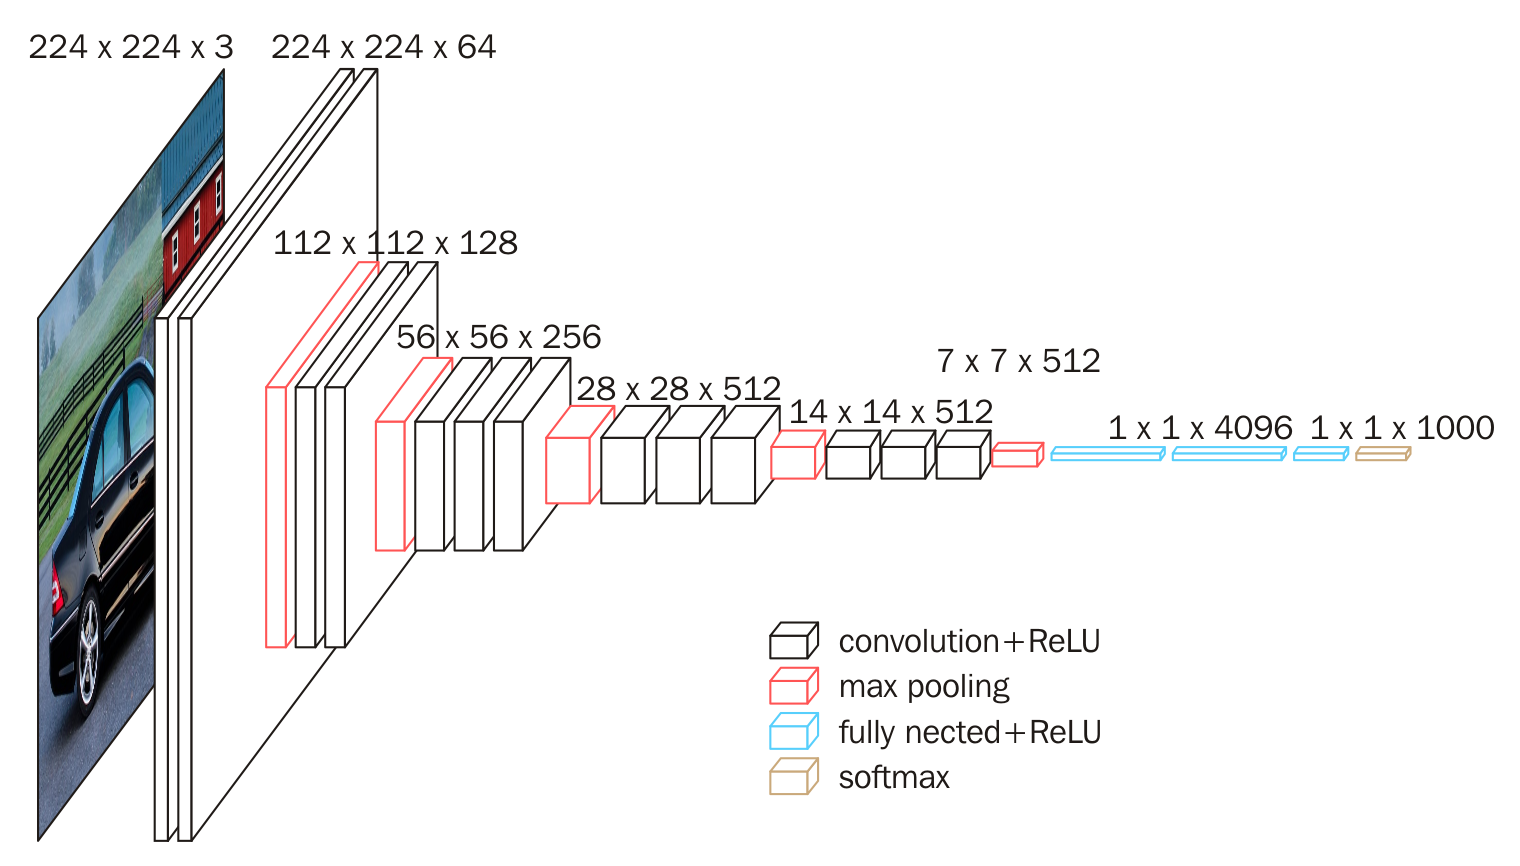
\includegraphics[width=0.7\textwidth]{figures/VGG16.png}
      \caption{VGG16结构示意图}
      \label{fig:vgg16}
    \end{figure}

由此,在2014年ImageNet大规模视觉识别挑战赛上牛津大学基于AlexNet网络提出VGG架构。相对于AlexNet网络,VGG减少了其卷积核的大小。它利用3个\(3\times3\)的卷积核来替代\(7\times7\)的卷积核,使用了2个\(3\times3\)的卷积核替代了\(5\times5\)的卷积核\cite{simonyan2014very}。这种小型的卷积核而不是大型卷积核可以保持更好的图像的性质,VGG16(图\ref{fig:vgg16})就是一种最经典的的VGG网络。

\subsection{VGG16网络结构及特点}
     \begin{figure}[h]
      \centering
      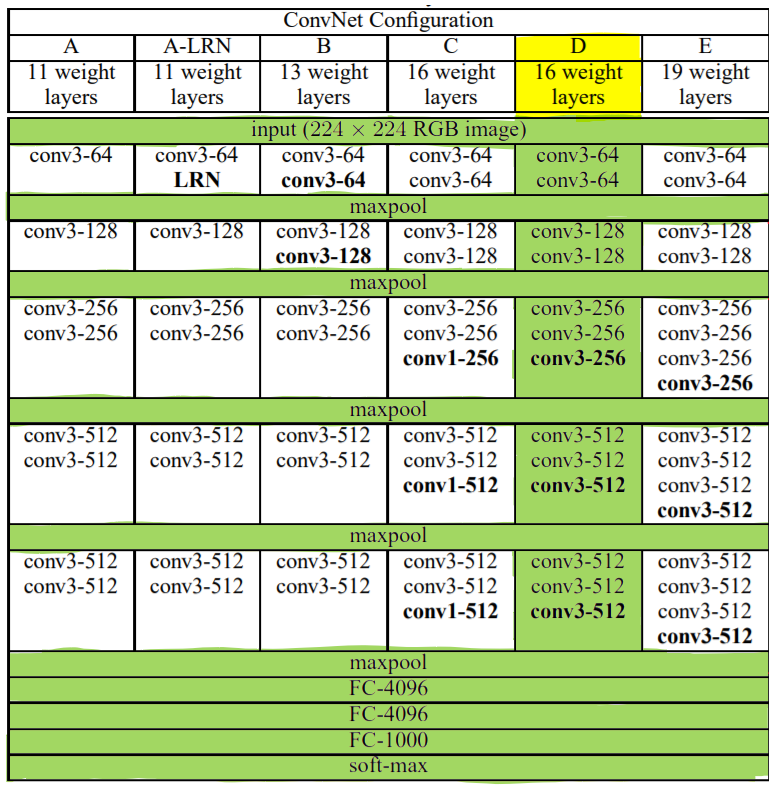
\includegraphics[width=0.6\textwidth]{figures/VGG2.png}
      \caption{VGG常见结构配置}
      \label{fig:vgg2}
    \end{figure}
根据卷积神经网络中卷积核和卷积层数目的不同,如图\ref{fig:vgg2}所示VGG共有六种常见的结构,其中后面两种结构的使用场景最多也最经典。D结构就是本节主要介绍的VGG16


通过对VGG16的结构进行具体分析,其组织结构一共包含以下层:

\begin{itemize}
    \item13层卷积层,在表中以conv3-YYY标号
    \item3层全连接层,在表中以FC-YYY标号
    \item5层池化层,在表中以maxpool标号
\end{itemize}

其中,权重层为卷积层和全连接层,总共有16层,因此此种结构被称为VGG16。

VGG网络的最大特点就是在于简单,因为把所有的大卷积核都缩小为\(3\times3\)的尺寸,并且按照若干层卷积层加上一层池化层的折叠方式,网络结构容易拟合。但是同时VGG16的权重参数有1亿多个,训练和调参难度过大,所以本文直接调用利用YouTube音频数据训练的网络VGGlish提取参数。

